\documentclass[11pt]{article}
\usepackage[margin=1in]{geometry}
\usepackage{fontspec,booktabs,array,graphicx,adjustbox,amsmath}
\usepackage[font=small,labelfont=bf]{caption}
\usepackage{natbib,xurl}
\usepackage[hidelinks]{hyperref}
\usepackage{setspace}
\setstretch{1.15}
\graphicspath{{../figs/}}
\newcommand{\YgWeightedTraitCI}{[0.1, 6.3]}
\newcommand{\MtRepOutN}{62}
\newcommand{\MtRepN}{172}
\newcommand{\YgCompleteWeightedN}{733}
\newcommand{\YgUnbiasedSameBias}{34}
\newcommand{\YgRaw}{1,500}
\newcommand{\YgWeightedFtCI}{[-1.9, 6.1]}
\newcommand{\MtRepOutCI}{[-5.3, 20.5]}
\newcommand{\YgInFtN}{739}
\newcommand{\YgUnalignedN}{51}
\newcommand{\YgUnbiasedLessBias}{37}
\newcommand{\YgInTraitControl}{63.5}
\newcommand{\YgWeightedTraitEstimate}{3.2}
\newcommand{\MtOutPermutationP}{0.654}
\newcommand{\MtAttention}{891}
\newcommand{\MtAssigned}{919}
\newcommand{\YgInTraitEstimate}{1.9}
\newcommand{\YgCompleteTraitCI}{[-1.0, 4.8]}
\newcommand{\MtOutEstimate}{1.2}
\newcommand{\MtAllInCI}{[-7.7, 1.4]}
\newcommand{\YgTraitInfluence}{[2.34, 2.69]}
\newcommand{\MtAsymmetryN}{583}
\newcommand{\MtDemN}{552}
\newcommand{\MtAsymmetryP}{0.120}
\newcommand{\YgOutTraitControl}{28.6}
\newcommand{\MtAttentionDrop}{39}
\newcommand{\YgCompleteTraitEstimate}{1.9}
\newcommand{\MtDemOutCI}{[-6.5, 5.0]}
\newcommand{\YgIndependentN}{316}
\newcommand{\YgInTraitCI}{[-0.9, 4.6]}
\newcommand{\MtN}{724}
\newcommand{\YgRepN}{492}
\newcommand{\YgUnbiasedMoreBias}{10}
\newcommand{\MtOutCI}{[-4.1, 6.5]}
\newcommand{\YgCompleteWeightedEstimate}{2.6}
\newcommand{\YgBiasedLessBias}{17}
\newcommand{\YgFtBound}{[-10.5, 13.3]}
\newcommand{\MtAllInEstimate}{-3.1}
\newcommand{\YgCompleteN}{1,088}
\newcommand{\YgTraitMissing}{8}
\newcommand{\YgBiasedSameBias}{46}
\newcommand{\YgN}{1,133}
\newcommand{\MtInN}{302}
\newcommand{\YgInFtPermutationP}{0.368}
\newcommand{\MtInP}{0.062}
\newcommand{\YgOutFtPermutationP}{0.766}
\newcommand{\MtDemOutEstimate}{-0.8}
\newcommand{\YgDemN}{641}
\newcommand{\YgFtMissing}{132}
\newcommand{\YgOutFtControl}{18.5}
\newcommand{\YgCompleteWeightedCI}{[-0.5, 5.8]}
\newcommand{\MtInCI}{[-8.9, 0.2]}
\newcommand{\YgOutFtCI}{[-2.8, 3.9]}
\newcommand{\MtInEstimate}{-4.3}
\newcommand{\YgInTraitN}{756}
\newcommand{\YgInTraitP}{0.180}
\newcommand{\YgOutTraitCI}{[-0.3, 5.4]}
\newcommand{\MtRepOutEstimate}{7.6}
\newcommand{\YgOutTraitN}{752}
\newcommand{\YgOutFtP}{0.764}
\newcommand{\YgOutTraitP}{0.081}
\newcommand{\MtInPermutationP}{0.062}
\newcommand{\YgOutTraitEstimate}{2.5}
\newcommand{\YgOutTraitPermutationP}{0.084}
\newcommand{\YgInFtControl}{66.5}
\newcommand{\YgInFtEstimate}{1.5}
\newcommand{\MtRaw}{930}
\newcommand{\YgInFtCI}{[-1.8, 4.9]}
\newcommand{\MtAsymmetryEstimate}{5.5}
\newcommand{\MtOutN}{281}
\newcommand{\MtOutP}{0.656}
\newcommand{\MtUnassigned}{11}
\newcommand{\MtRepOutP}{0.241}
\newcommand{\YgCompleteWeightedP}{0.100}
\newcommand{\YgWeightedFtEstimate}{2.1}
\newcommand{\MtAllInN}{315}
\newcommand{\YgBiasedMoreBias}{16}
\newcommand{\MtAllInP}{0.180}
\newcommand{\YgInFtP}{0.363}
\newcommand{\YgWeightedFtN}{667}
\newcommand{\YgWeightedFtP}{0.310}
\newcommand{\YgInTraitPermutationP}{0.177}
\newcommand{\YgWeightedTraitN}{752}
\newcommand{\YgWeightedTraitP}{0.045}
\newcommand{\YgOutFtN}{667}
\newcommand{\MtDemOutN}{219}
\newcommand{\MtDemOutP}{0.785}
\newcommand{\MtAsymmetryCI}{[-1.4, 12.5]}
\newcommand{\YgCompleteTraitN}{733}
\newcommand{\YgTraitBound}{[1.3, 3.8]}
\newcommand{\YgCompleteTraitP}{0.193}
\newcommand{\YgTraitCategory}{0.10}
\newcommand{\YgOutFtEstimate}{0.5}

\title{Principled Partisan Affect?\\Evidence from Two Survey Experiments}
\author{Douglas J. Ahler \and Carolyn E. Roush \and Gaurav Sood}
\date{}
\begin{document}
\maketitle
\begin{abstract}
\noindent Partisans might dislike their opponents partly because they regard them as biased. If so, portraying opponents as fair-minded could soften that dislike, while portraying one's own side as biased could erode its appeal. We examine these possibilities in two survey experiments. In a 2013 MTurk study, declining rather than sustained approval of a party leader after a controversy changed own-party warmth by \MtInEstimate{} points on a 0--100 scale (95\% CI \MtInCI{}); the opposition estimate was \MtOutEstimate{} (\MtOutCI{}). In a 2018 YouGov study, an article portraying the opposition as fair-minded raised favorable trait ratings by \YgOutTraitEstimate{} points (\YgOutTraitCI{}), but changed warmth by only \YgOutFtEstimate{} (\YgOutFtCI{}). An article portraying one's own party as biased produced no clear penalty. The trait result is suggestive: its precision depends on weighting and item completeness. The experiments identify responses to particular news stories, whose features extend beyond attributed reasoning. The YouGov design also confounds the target's partisan relationship with its portrayed behavior. The evidence therefore supports neither a general claim that partisans reward fair-mindedness nor a demonstrated partisan double standard.
\end{abstract}

\section{The question}
Dislike of the other party need not arise solely from disagreement about policy. Partisans also judge the people on the other side, often unfavorably \citep{iyengar2012}. One possible basis for such judgments is a perceived failure to reason fairly: opponents appear willing to defend their leaders regardless of the evidence. If this perception contributes to animus, showing opponents behaving fairly might improve evaluations of them. The same standard, applied consistently, would make evidence of bias among one's own allies a reason to like them less.

There is a competing possibility. Partisans may prefer loyalty to their own side while condemning it in their opponents. Evidence of declining support for one's own leader could then reduce affection for fellow partisans, even when the decline follows a controversy. Evidence of sustained support might reassure rather than repel. These accounts concern responses to representations of others' behavior. They do not require that the representations be accurate or that respondents actually engage in fair or biased reasoning themselves.

The distinction matters for interpreting a bias blind spot. Evidence that people see more bias in others than in themselves \citep{pronin2002} does not by itself establish that they use different standards for their own party and its opposition. That is an additional hypothesis. News portrayals can affect political judgments: \citet{levendusky2016}, for example, find that coverage emphasizing partisan polarization increases dislike of the opposition. Whether portrayals of reasoning quality have comparable consequences is an empirical question.

We bring two experiments to this question. The first varied a party's reported approval of its leader after a controversy. The second contrasted articles portraying opponents as fair-minded or allies as biased with a control story. The evidence is limited. There is a small, uncertain improvement in trait ratings of supposedly fair-minded opponents, but little corresponding movement in warmth. Neither the research design nor the estimates establish the psychological mechanism or a partisan double standard.

\section{Design and estimands}
The studies differ in recruitment, stimuli, measurement, and the comparisons they permit. We analyze each separately. In both, the unit is the respondent, party leaners are included with their party, and the outcomes are measured immediately after the article. The reported intervals are two-sided 95\% intervals. These are exploratory analyses of completed studies; we found no preregistered analysis plan in the study materials.

For each comparison, we estimate the treatment difference separately among Democrats and Republicans and average the differences using their shares in the study's full eligible partisan sample. If $p$ indexes party, $s_p$ is that share, and $a$ and $b$ are the compared arms, the estimand is
\[
\widehat\tau=\sum_p s_p(\overline Y_{pa}-\overline Y_{pb}).
\]
This prevents differences in the party composition of the realized arms from changing the pooled comparison. Each outcome uses the respondents who answered it; the standardization shares remain fixed across outcomes. Unweighted intervals use the sum of independent cell-mean variances and Welch--Satterthwaite degrees of freedom. The supplemental weighted estimates treat the supplied weights as fixed, use within-cell weighted means and HC3 variances, and standardize to weighted party shares. They address a different population composition from the unweighted estimates.

The questionnaires describe random allocation among eligible articles. The delivered assignments agree with their partisan routing. We do not have the randomizer's execution logs. Causal readings require the stated randomization to have been implemented, the assigned stories to have been delivered, no interference between respondents, and an adequate account of outcome nonresponse. Random assignment identifies an effect of an article package. It does not identify a separate effect of perceived bias when other article features change too.

\section{Declining support after controversy: MTurk, 2013}
The first experiment was fielded on Amazon Mechanical Turk in November 2013. The source file contains \MtRaw{} records, of which \MtAssigned{} have a known article assignment. The \MtUnassigned{} records without assignment also lack the two party thermometers; we do not treat them as an assigned control group. Before treatment, an attention question instructed respondents to select only blue and yellow. Requiring those choices and no others excludes \MtAttentionDrop{} records. The main sample consists of \MtN{} assigned partisans passing this check: \MtDemN{} Democrats and \MtRepN{} Republicans. This convenience sample is not representative of American adults.

Respondents received one of five researcher-modified news stories: two about Democrats' approval of Barack Obama after controversies surrounding his administration, two about Republicans' approval of Ted Cruz after the government shutdown, and a control about support for Toronto mayor Rob Ford despite his drug scandal. Within each American party's stories, approval either declined or remained high. ``Sustained'' describes the latter condition; its reported approval rose slightly rather than remaining numerically identical. Approval levels, trajectories, quotations, and accompanying narrative differed across the variants. We therefore compare versions of a story rather than treating the manipulation as a pure change in reasoning quality.

The main contrasts compare declining with sustained approval of the same leader. The outcome is a 0--100 feeling thermometer for Democrats or Republicans, oriented to the respondent's own party or the opposition. Randomly ordered outcome blocks are combined only after checking that overlapping responses do not conflict. Every record with a known article assignment has both thermometers. Comparisons with the Ford control, shown in the appendix, additionally change the leader, party context, and controversy.

\begin{figure}[!htbp]
\centering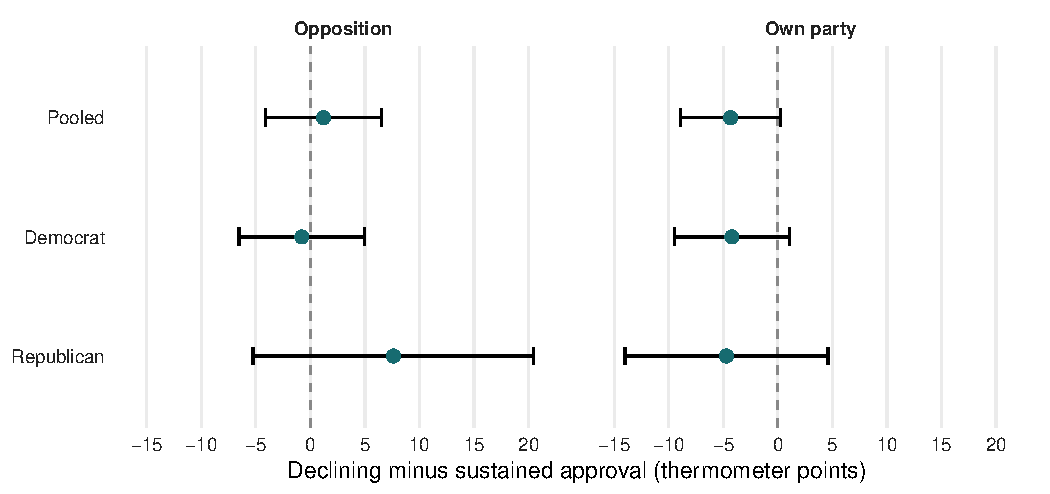
\includegraphics[width=\linewidth]{mturk_effects.pdf}
\caption{MTurk: declining rather than sustained approval after controversy. Points are differences in warmth toward the party described; bars are 95\% Welch intervals. The pooled estimates standardize to the party composition of the \MtN{} eligible respondents. Each contrast uses only the two relevant article arms.}
\label{fig:mt}
\end{figure}

Declining support for one's own leader did not produce a clear reward for holding that leader accountable. The estimated change in own-party warmth is \MtInEstimate{} points (\MtInCI{}; Figure~\ref{fig:mt}). Its direction is consistent with a preference for continued support, but the interval includes little or no change. For the opposition, the estimate is \MtOutEstimate{} (\MtOutCI{}). The difference between these two effects is \MtAsymmetryEstimate{} points (\MtAsymmetryCI{}). Thus the data do not establish that the response differs according to whether the story concerns allies or opponents.

The party-specific estimates are less precise. The opposition contrast is \MtDemOutEstimate{} among Democrats (\MtDemOutCI{}) and \MtRepOutEstimate{} among Republicans (\MtRepOutCI{}). The contrast between an imprecise positive estimate and an imprecise near-zero estimate is not itself evidence of a party difference. Removing the attention exclusion also weakens the negative own-party estimate (Appendix Table~\ref{tab:mtattention}). The pilot offers a possible loyalty response to these stories, with substantial uncertainty, rather than a general demonstration that partisans punish fair-mindedness.

\section{Portraying allies and opponents: YouGov, 2018}
YouGov fielded the second study from May 11 to May 29, 2018. Its codebook reports 1,596 interviews, from which 1,500 respondents were matched on gender, age, race, and education; subsequent weighting used propensity calibration and presidential vote. These are the vendor's recruitment and adjustment procedures, not probability sampling. The delivered file contains \YgRaw{} records. We report unweighted experimental comparisons first and weighted estimates as a sensitivity analysis. Interpreting either as an effect for all American adults requires assumptions about selection and treatment-effect generalization.
% Interview counts and field dates above come from data/materials/yougov/codebook.pdf, not an analysis estimate.

The party measure used before assignment identifies \YgDemN{} Democrats and \YgRepN{} Republicans, including leaners, for a main sample of \YgN{} partisans. There are also \YgIndependentN{} independents and \YgUnalignedN{} respondents selecting ``not sure.'' They have no defined own-versus-opposition party in our analysis and are reported separately in the appendix. We use the pre-assignment party measure to define the main sample and orient outcomes.

\begin{table}[!htbp]
\centering
\caption{The three arms available to each partisan group in YouGov.}
\label{tab:assignment}
\adjustbox{max width=\linewidth}{\begin{tabular}{lrrr}
\toprule
Respondents & Control & Fair-minded opposition & Biased own party \\
\midrule
Democrats & 217 & 210 & 214 \\
Republicans & 166 & 164 & 162 \\
\bottomrule
\end{tabular}
}
\begin{minipage}{\linewidth}\footnotesize
The portrayed party depends on the respondent's pre-assignment party. Democrats could read about fair-minded Republicans or biased Democrats; Republicans could read about fair-minded Democrats or biased Republicans.
\end{minipage}
\end{table}

Each partisan was eligible for a control article, an article portraying the opposition as fair-minded, or an article portraying their own party as biased (Table~\ref{tab:assignment}). The fair-minded articles described economic evaluations that remained stable across the transition from Obama to Trump and included favorable expert commentary. The biased articles described economic evaluations shifting after the election and included disparaging commentary from a political opponent. The control described aggregate economic views. The articles also differed in dates, framing, sources, and party references. These are experimental materials, not verified news reports or evidence that the depicted partisans actually reasoned well or poorly. Economic expectations can rationally change when the presidency changes; a change in expectations alone is not a sufficient test of bias.

Crucially, partisans were never assigned to fair-minded-own-party or biased-opposition articles. The design therefore cannot estimate the effect of the same portrayal for both partisan targets. Comparing the two available treatment effects changes both the target and the portrayal. Calling that difference a partisan double standard would exceed what was randomized.

\subsection{Two distinct outcomes}
The feeling thermometers rate the Democratic Party and Republican Party from 0 to 100. The pilot instead named Democrats and Republicans. We do not treat these as identical objects of evaluation or combine the studies' estimates.

The trait battery asks how well each of six descriptions fits each party: ignorant, sincere, open to reason, smug, patriotic, and hypocritical. Responses run from very poorly to very well. We reverse the three unfavorable descriptions and average available answers, rescaling the mean to 0--100. Higher values indicate more favorable judgments. This equally weighted index summarizes the measured descriptions; it is not a validated latent measure of fair-mindedness. A one-category shift on every constituent item would change the index by 25 points. The questionnaire includes a selfishness item that is absent from the delivered data, so it is not part of the index.

There are \YgFtMissing{} missing opposition thermometers among the main sample, compared with \YgTraitMissing{} wholly missing opposition trait indices. Only \YgCompleteN{} respondents answer all six opposition trait items. We report response counts by arm, complete-item estimates, and bounded-outcome sensitivity below. Conditioning on an observed outcome can compromise a randomized comparison if response depends on treatment and potential evaluations. Similar response rates alone would not resolve that concern.

\subsection{Results}
An article portraying opponents as fair-minded produces a small favorable shift in their trait ratings, but little change in warmth. The trait estimate is \YgOutTraitEstimate{} points (95\% CI \YgOutTraitCI{}), relative to a standardized control mean of \YgOutTraitControl{}. This is equivalent to \YgTraitCategory{} of a response category averaged across the constituent items. The warmth estimate is \YgOutFtEstimate{} points (\YgOutFtCI{}), relative to a control mean of \YgOutFtControl{}. The intervals permit modest improvements and some deterioration; a near-zero point estimate is not proof of no effect.

\begin{figure}[!htbp]
\centering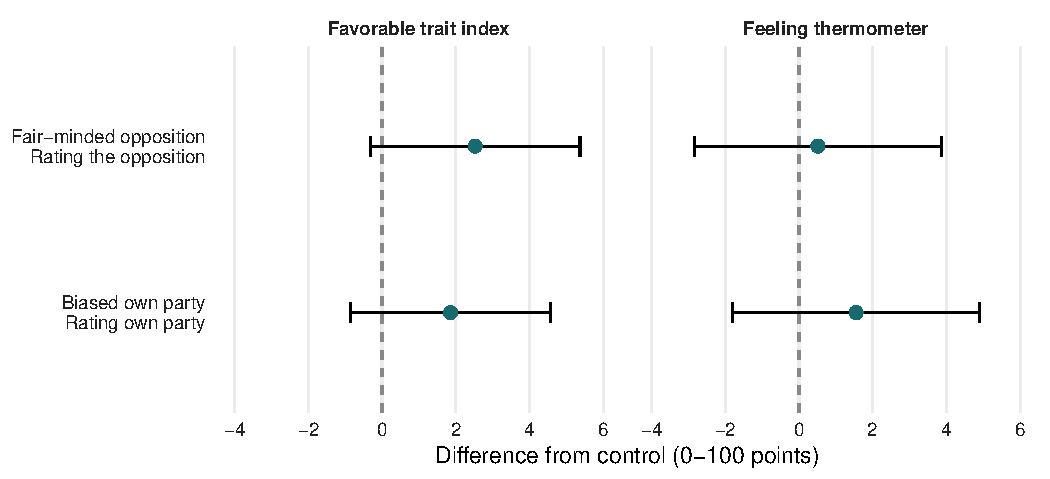
\includegraphics[width=\linewidth]{yougov_effects.pdf}
\caption{YouGov: responses to portrayals of the opposition and one's own party. Differences from control, standardized to the eligible partisan composition. Bars are 95\% Welch intervals. The two panels measure different judgments on a common 0--100 reporting scale.}
\label{fig:yg}
\end{figure}

\begin{table}[!htbp]
\centering\small
\caption{YouGov primary comparisons.}
\label{tab:yg}
\adjustbox{max width=\linewidth}{\begin{tabular}{llrrr}
\toprule
Article / rated target & Measure & Control & Difference [95\% CI] & $n$ \\
\midrule
Fair-minded opposition & Warmth & 18.5 & 0.5 [-2.8, 3.9] & 667 \\
Fair-minded opposition & Traits & 28.6 & 2.5 [-0.3, 5.4] & 752 \\
Biased own party & Warmth & 66.5 & 1.5 [-1.8, 4.9] & 739 \\
Biased own party & Traits & 63.5 & 1.9 [-0.9, 4.6] & 756 \\
\bottomrule
\end{tabular}
}
\begin{minipage}{\linewidth}\footnotesize
Control means and differences are standardized over pre-assignment party. $n$ counts observed outcomes in the two compared arms, not the full three-arm sample. ``Traits'' is the available-item favorable index. All outcomes run from 0 to 100. Intervals are unadjusted for multiple comparisons.
\end{minipage}
\end{table}

The article portraying one's own party as biased does not yield a clear penalty. Its estimates are \YgInFtEstimate{} points for warmth (\YgInFtCI{}) and \YgInTraitEstimate{} for traits (\YgInTraitCI{}). Their positive signs should not be turned into a demonstrated reward for bias: both intervals include negative and positive effects, and the article bundles several changes. None of the four main YouGov comparisons, or the two pilot comparisons, rejects a zero effect at the conventional 5\% level after Holm adjustment within study. That accounting does not make all effects zero, but it rules out presenting the most favorable comparison as an isolated confirmatory result.

\subsection{Sensitivity and missing outcomes}
The trait result varies with the weighting and completeness decisions (Figure~\ref{fig:sensitivity}). Survey weighting raises the estimated opposition trait effect to \YgWeightedTraitEstimate{} (\YgWeightedTraitCI{}). Requiring all six items gives \YgCompleteTraitEstimate{} (\YgCompleteTraitCI{}) without weights and \YgCompleteWeightedEstimate{} (\YgCompleteWeightedCI{}) with weights. The weighted warmth estimate is \YgWeightedFtEstimate{} (\YgWeightedFtCI{}). The point estimates favor a small trait improvement, but their precision does not support a specification-independent declaration of a positive effect. The item estimates in the appendix also show why the composite should not be equated with a single judgment of hypocrisy.

\begin{figure}[!htbp]
\centering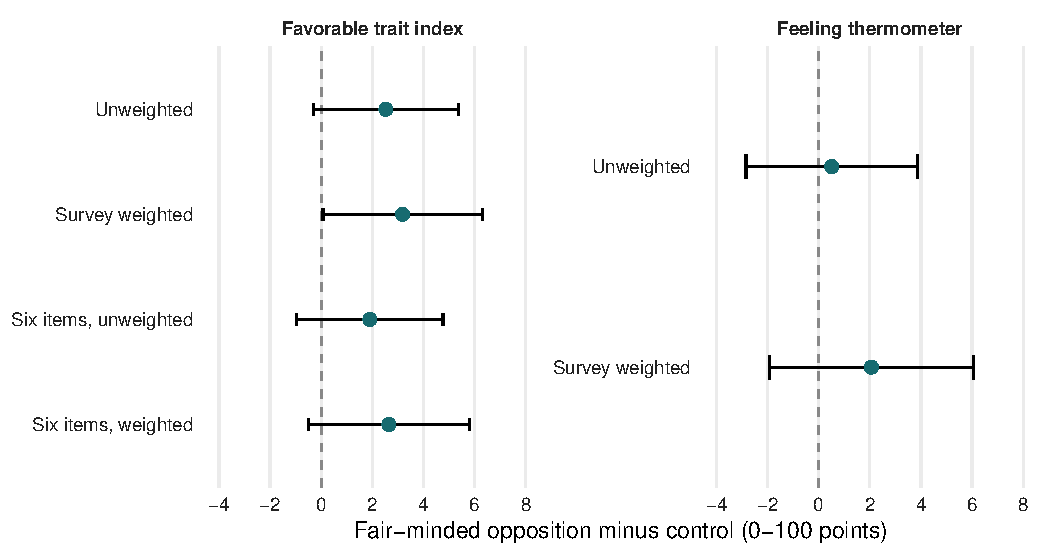
\includegraphics[width=\linewidth]{sensitivity.pdf}
\caption{YouGov opposition effects under weighting and item-completeness choices. Bars are 95\% intervals: stratified Welch for unweighted estimates and fixed-weight HC3 for weighted estimates. Complete-item analysis also selects a different set of respondents. Weighted and unweighted estimates standardize to their respective eligible party shares.}
\label{fig:sensitivity}
\end{figure}

The warmth result is particularly exposed to missing outcomes. Assigning every missing thermometer either endpoint of its scale gives worst-case bounds of \YgFtBound{} for the full-sample opposition contrast. Applying the same exercise separately to every missing constituent trait answer gives \YgTraitBound{} for the fixed six-item mean. These are ranges over possible completions of this dataset, not sampling confidence intervals. The positive lower trait bound describes the realized completed-data contrast; it does not remove randomization uncertainty or prove a positive population effect. The thermometer bounds are much wider and show that observed-case estimates alone do not sharply locate its full-sample effect.

No single observed respondent drives the available-item trait estimate: holding the party standardization fixed, deleting one respondent at a time yields estimates from \YgTraitInfluence{}. A permutation check that shuffles assignment within party among respondents with observed outcomes gives $p=\YgOutTraitPermutationP{}$ for this contrast. This check is conditional on outcome observation; it is not a remedy for treatment-dependent missingness.

\section{What the experiments establish}
The two studies do not deliver a consistent reward for apparently fair-minded partisans or a consistent penalty for apparent bias. The pilot's own-party estimate is negative when approval of the leader declines, although imprecise and sensitive to the attention rule. The later experiment suggests a small improvement in favorable descriptions of fair-minded opponents, with little corresponding movement in warmth. Judging a party somewhat more favorably on selected traits and feeling warmer toward it are distinguishable responses.

There are several reasons to resist a stronger theoretical conclusion. The pilot manipulates reported approval and the later experiment manipulates accounts of economic evaluations. Neither isolates reasoning quality from approval levels, commentary, or other content. The later study lacks the cells needed to compare identical behavior by allies and opponents. Post-article manipulation checks cannot turn these packages into an identified mediation design. Nor can short-run self-reports establish how people behave toward opponents or how enduring partisan animus develops.

A sharper test would independently randomize the partisan target and the evidence of fair or biased reasoning, hold the surrounding story constant, and measure both perceived reasoning and subsequent affect with adequate power and follow-up. The present findings motivate that test. They do not settle whether partisan affect is principled.

\section*{Data and replication}
The replication materials are available at \url{https://github.com/soodoku/principled}. They include deidentified respondent data, study materials, the complete R analysis, generated estimates, and this manuscript. Original source files are retained separately. \texttt{make check} reproduces the paper and runs linting and tests. The data documentation specifies exclusions, coding, missing values, inference, and the optional export from original files.

\bibliographystyle{apalike}
\bibliography{references}
\clearpage
\appendix
\section{Supplementary comparisons}
The tables below preserve the distinction between an eligible sample and the respondents contributing to a particular observed-outcome comparison. Party-specific estimates use their own group's observed cell means; the pooled estimates in the text instead standardize to both parties' shares.

\begin{table}[!htbp]
\centering\small
\caption{MTurk attention rules: declining minus sustained approval.}
\label{tab:mtattention}
\adjustbox{max width=\linewidth}{\begin{tabular}{lrr}
\toprule
Sample & Own party & Opposition \\
\midrule
Strict attention & -4.3 [-8.9, 0.2] & 1.2 [-4.1, 6.5] \\
No attention exclusion & -3.1 [-7.7, 1.4] & 1.4 [-3.9, 6.6] \\
Loose attention & -4.1 [-8.7, 0.5] & 1.2 [-4.1, 6.5] \\
\bottomrule
\end{tabular}
}
\begin{minipage}{\linewidth}\footnotesize
Entries are thermometer differences with 95\% Welch intervals. Strict attention requires only the two requested colors; loose attention allows additional choices. All rules use known assignments and partisan identification. The party shares are recalculated for each eligible sample.
\end{minipage}
\end{table}

\begin{table}[!htbp]
\centering\small
\caption{MTurk stories compared with the Ford control, by respondent party.}
\adjustbox{max width=\linewidth}{\begin{tabular}{lrr}
\toprule
Target & Decline versus Ford & Sustained versus Ford \\
\midrule
\multicolumn{3}{l}{\textit{Democrat respondents}} \\
Own party & -5.3 [-10.6, -0.0] & -1.1 [-6.4, 4.2] \\
Opposition & 0.4 [-4.7, 5.6] & 1.2 [-4.7, 7.1] \\
\multicolumn{3}{l}{\textit{Republican respondents}} \\
Own party & -3.3 [-12.7, 6.1] & 1.4 [-8.7, 11.5] \\
Opposition & 6.6 [-5.7, 19.0] & -1.0 [-11.1, 9.2] \\
\bottomrule
\end{tabular}
}
\begin{minipage}{\linewidth}\footnotesize
Entries are differences in thermometer ratings, with 95\% Welch intervals. These comparisons change the leader, national and partisan context, and controversy, as well as the described approval pattern. They do not isolate approval decline.
\end{minipage}
\end{table}

\begin{table}[!htbp]
\centering\small
\caption{YouGov response counts: observed / assigned.}
\adjustbox{max width=\linewidth}{\begin{tabular}{lrrr}
\toprule
Target / measure & Control $n$ & Fair-minded $n$ & Biased $n$ \\
\midrule
Opposition warmth & 343/383 & 324/374 & 334/376 \\
Opposition traits & 381/383 & 371/374 & 373/376 \\
Opposition traits: six items & 374/383 & 359/374 & 355/376 \\
Own-party warmth & 374/383 & 367/374 & 365/376 \\
Own-party traits & 381/383 & 371/374 & 375/376 \\
\bottomrule
\end{tabular}
}
\begin{minipage}{\linewidth}\footnotesize
Assigned counts include all eligible partisans. Trait indices use any available item unless marked ``six items.'' Each main effect compares one treatment arm with control. Respondents in the other arm do not contribute to that contrast's reported $n$.
\end{minipage}
\end{table}

\clearpage
\begin{table}[!htbp]
\centering\small
\caption{YouGov effects by respondent party.}
\adjustbox{max width=\linewidth}{\begin{tabular}{llrr}
\toprule
Article & Outcome & Democrats & Republicans \\
\midrule
Fair-minded opposition & Opposition warmth & 0.9 [-3.6, 5.5] & -0.0 [-5.0, 4.9] \\
Fair-minded opposition & Opposition traits & 2.1 [-1.7, 5.8] & 3.1 [-1.3, 7.5] \\
Fair-minded opposition & Own-party warmth & -2.3 [-6.7, 2.2] & 6.0 [0.7, 11.2] \\
Fair-minded opposition & Own-party traits & 0.3 [-3.3, 3.8] & 3.3 [-0.8, 7.3] \\
Fair-minded opposition & Warmth gap & -2.6 [-9.5, 4.2] & 4.0 [-3.4, 11.4] \\
Biased own party & Opposition warmth & -1.9 [-6.3, 2.5] & 3.2 [-2.0, 8.4] \\
Biased own party & Opposition traits & -0.2 [-3.8, 3.4] & 0.9 [-3.3, 5.2] \\
Biased own party & Own-party warmth & -0.5 [-4.8, 3.9] & 4.2 [-1.1, 9.4] \\
Biased own party & Own-party traits & -0.2 [-3.8, 3.5] & 4.5 [0.3, 8.6] \\
Biased own party & Warmth gap & 2.6 [-4.4, 9.6] & -0.1 [-7.3, 7.1] \\
\bottomrule
\end{tabular}
}
\begin{minipage}{\linewidth}\footnotesize
Unweighted differences from control with 95\% Welch intervals. Outcomes run from 0 to 100 except the warmth gap, defined as own-party minus opposition warmth, which runs from $-100$ to 100. Effects on the party not described and on the gap are secondary comparisons. Comparing the significance of two estimates is not a test of their difference.
\end{minipage}
\end{table}

\begin{figure}[!htbp]
\centering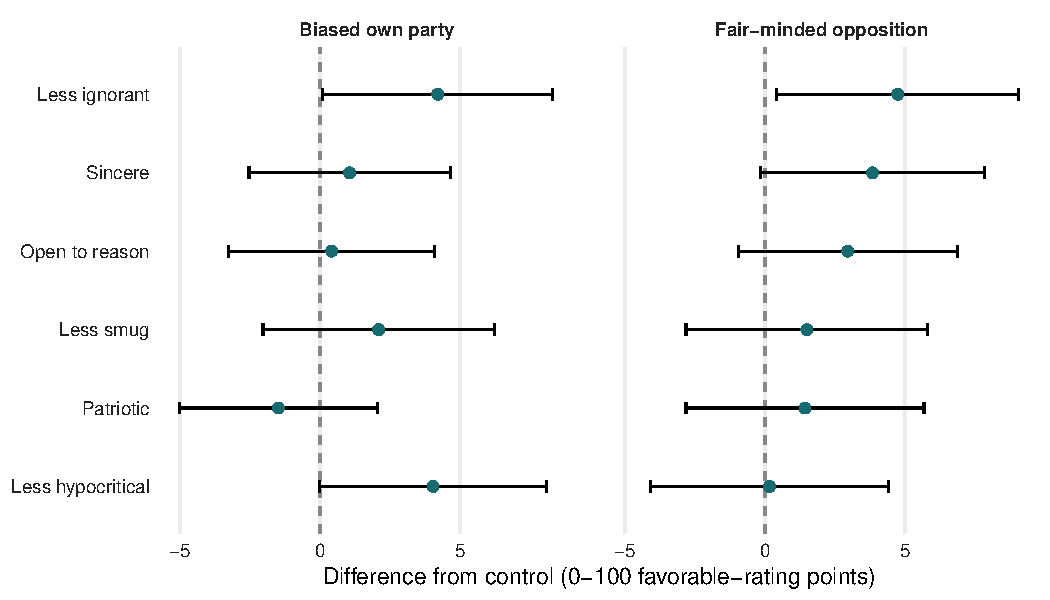
\includegraphics[width=\linewidth]{trait_items.pdf}
\caption{YouGov constituent traits. Unweighted differences from control; 95\% Welch intervals. Unfavorable descriptions are reversed so that positive values always mean more favorable ratings. Intervals are not multiplicity-adjusted; the replication output also reports Holm-adjusted $p$-values across the item comparisons.}
\end{figure}

\clearpage
\begin{table}[!htbp]
\centering\small
\caption{YouGov respondents without a partisan side: evaluations of Republicans.}
\adjustbox{max width=\linewidth}{\begin{tabular}{llrr}
\toprule
Respondents & Article & Republican traits & Republican warmth \\
\midrule
Independent & unbiased & 5.6 [0.3, 10.9] & 4.8 [-2.3, 11.9] \\
Independent & biased & 2.3 [-3.6, 8.2] & 2.0 [-5.5, 9.4] \\
Not sure & unbiased & -13.2 [-25.3, -1.1] & -3.0 [-24.3, 18.3] \\
Not sure & biased & -4.0 [-12.5, 4.6] & -7.6 [-27.7, 12.5] \\
\bottomrule
\end{tabular}
}
\begin{minipage}{\linewidth}\footnotesize
Unweighted differences from control with 95\% Welch intervals. ``Unbiased'' is the fair-minded-Republican article, and ``biased'' the biased-Republican article. Independents and respondents answering ``not sure'' to pre-assignment party identification are separate groups. The observed routing for ``not sure'' matches that for independents, but the questionnaire does not explicitly document that routing. These estimates concern Republican evaluations, not out-party affect.
\end{minipage}
\end{table}

\section{Computation and scope of uncertainty}
For the primary unweighted estimates, let $s^2_{pa}$ and $n_{pa}$ be the sample variance and observed count in party--arm cell $(p,a)$, and let $c_a$ encode the arm contrast. The estimated variance is
\[
\widehat V(\widehat\tau)=\sum_{p,a}s_p^2 c_a^2\frac{s^2_{pa}}{n_{pa}}.
\]
Writing each summand as $v_{pa}$, the Welch degrees of freedom are $(\sum v_{pa})^2/\sum[v_{pa}^2/(n_{pa}-1)]$. This calculation conditions on the standardization shares and treats respondents as independent. It does not include uncertainty from sample recruitment or the selection of these particular stimuli.

For a weighted cell, normalized weights are $h_i=w_i/\sum_iw_i$. Its HC3 variance is $\sum_i\{h_i(Y_i-\overline Y_w)/(1-h_i)\}^2$. We combine these cell variances with the squared weighted party shares and contrast coefficients, using observed comparison size minus the number of compared cells as the reference $t$ degrees of freedom. The supplied weights' estimation uncertainty is not included. No geographic or household cluster identifiers needed for a different dependence model are available in the public analysis data.

The replication tables also retain raw cell means, effective cell sample sizes, response-rate contrasts, all main outcome comparisons under both weighting choices, leave-one-item-out indices, exact case-deletion ranges, and the seeded permutation checks. These checks probe the reported estimator and selected analytic choices. They do not compensate for absent treatment cells, validate the news stories, or establish an unmeasured mechanism.
\end{document}
